% Fig. 2: panel a (matplotlib PDF, included at 100%) and panel b, the reservoir, drawn here.
% Width 7.05 in = 17.907 cm, height 2.375 in = 6.033 cm. Panel a has square axes and is 1.68 in = 4.267 cm wide; panel b
% is drawn at 1.078 times its original size (coordinates only: text, line widths and symbols keep their size), so that
% the reservoir carries the figure. Both titles sit 10.4 bp = 0.367 cm below the top, as in the matplotlib panels. The
% bottom row holds the formula of the task (under panel a) and the three legend boxes of panel b.
\documentclass[border=0pt]{standalone}
% Shared TikZ style for the schematics. Same typeface, size (8 pt) and palette as figstyle.py:
% blue = memory / reservoir dynamics, red = noise and the limit, purple = input, greys = neutral.
\usepackage[T1]{fontenc}
\usepackage{helvet}
\renewcommand{\familydefault}{\sfdefault}
\usepackage{amsmath,amssymb,bm}
\usepackage{tikz}
\usetikzlibrary{arrows.meta,calc,decorations.pathreplacing,patterns.meta,shapes.geometric,shadows}
\definecolor{cInk}{HTML}{1A1A1A}
\definecolor{cBlue}{HTML}{3C7FE0}
\definecolor{cBlueDark}{HTML}{1D4C9C}
\definecolor{cBlueLight}{HTML}{8DB8F0}
\definecolor{cBlueFill}{HTML}{DDE9F9}
\definecolor{cRed}{HTML}{EF4B3B}
\definecolor{cRedDark}{HTML}{B8301F}
\definecolor{cRedFill}{HTML}{FCE3DE}
\definecolor{cPurple}{HTML}{9B4FE0}
\definecolor{cPurpleDark}{HTML}{6B2CAB}
\definecolor{cPurpleFill}{HTML}{EFE2FB}
\definecolor{cGreyDark}{HTML}{4A4A4A}
\definecolor{cGrey}{HTML}{8C8C8C}
\definecolor{cGreyLight}{HTML}{B4B4B4}
\definecolor{cGreyFill}{HTML}{EDEDED}
\definecolor{cShadow}{HTML}{B5B5B5}
\tikzset{
  every node/.style={font=\fontsize{8}{9.6}\selectfont},
  lbl/.style={font=\fontsize{8}{9.6}\selectfont},
  ttl/.style={font=\fontsize{8}{9.6}\selectfont,anchor=base west,inner sep=0pt},
  ttlr/.style={font=\fontsize{8}{9.6}\selectfont,anchor=base east,inner sep=0pt},
  wire/.style={line width=0.65pt,cInk},
  ublk/.style={draw=cInk,line width=0.6pt,fill=cBlue,rounded corners=1.6pt},
  iblk/.style={draw=cInk,line width=0.6pt,rounded corners=1.6pt,preaction={fill=cPurple},
    pattern={Lines[angle=55,distance=2.2pt,line width=0.85pt]},pattern color=white},
  nbox/.style={draw=cInk,line width=0.55pt,fill=cRed,rounded corners=1.1pt},
  feat/.style={draw=cInk,line width=0.6pt,fill=white,rounded corners=2pt,inner sep=1.6pt,
    minimum width=0.98cm,minimum height=0.44cm},
  legbox/.style={draw=cInk,line width=0.8pt,fill=white,rounded corners=2.4pt,
    drop shadow={shadow xshift=1.2pt,shadow yshift=-1.2pt,fill=cShadow,opacity=1}},
  arr/.style={line width=0.65pt,-{Stealth[length=3.6pt,width=3.2pt]}},
  brc/.style={decorate,decoration={brace,amplitude=2.6pt},line width=0.55pt},
}
\newcommand{\Discard}[3][cInk]{%
  \draw[line width=0.75pt,#1] (#2,{#3-0.1}) -- (#2,{#3+0.1});
  \draw[line width=0.75pt,#1] ({#2+0.05},{#3-0.064}) -- ({#2+0.05},{#3+0.064});
  \draw[line width=0.75pt,#1] ({#2+0.1},{#3-0.03}) -- ({#2+0.1},{#3+0.03});}
\providecommand{\ket}[1]{|#1\rangle}
\providecommand{\nrm}[2]{\lvert #1\rvert_{#2}}

\begin{document}
\begin{tikzpicture}[x=1cm,y=1cm]
\useasboundingbox (0,0) rectangle (17.907,6.033);
\node[anchor=north west,inner sep=0pt,outer sep=0pt] at (0,6.033) {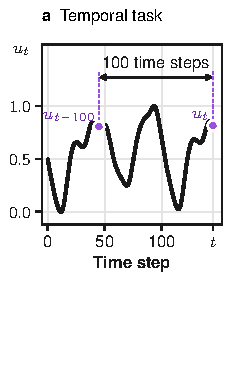
\includegraphics{fig2a.pdf}};
% formula of the task, in a box of the legend style, under panel a; the gap to the first legend box of panel b
% (0.18 cm) equals the gaps between the legend boxes
\path[legbox] (0.30,0.06) rectangle (4.25,0.901);
\node[align=center,inner sep=0pt] at (2.275,0.4805) {target of the forecast:\\[1pt]$y_{t+1}=0.7\,u_t+0.3\,u_{t-100}$};
% =================================================================================== panel b
\def\XB{4.427}\def\SB{1.078}
\node[ttl] at (\XB,5.666) {\textbf{b}\enspace Quantum reservoir computer};
% legend bottom (y = 0.06) stays 0.06 cm above the bottom edge: shift y by 0.06 (1 - s)
\begin{scope}[shift={(\XB,{0.06*(1-\SB)})},scale=\SB]
% ------------------------------------------------------------------ geometry
\def\yA{3.94}\def\yB{3.56}\def\yC{3.00}\def\yD{2.62}\def\yE{2.24}\def\yF{1.86}
\def\xL{2.12}\def\xR{8.65}
\def\sA{2.30}\def\sB{5.25}
% ------------------------------------------------------------------ wires
\foreach \y in {\yC,\yD,\yE,\yF} \draw[wire] (\xL,\y) -- (\xR,\y);
\foreach \y in {\yA,\yB} {
  \draw[wire] (\xL,\y) -- (\sA,\y);                 % previous input register, discarded at step t-1
  \draw[wire] ({\sA+0.62},\y) -- (\sB,\y);          % input register of step t-1, discarded at step t
  \draw[wire] ({\sB+0.62},\y) -- (\xR,\y);          % input register of step t
  \Discard{\sA}{\y} \Discard{\sB}{\y}
}
% ------------------------------------------------------------------ two time steps
\newcommand{\Blk}[3]{\path[ublk] ({#1-0.15},{#2+0.13}) rectangle ({#1+0.15},{#3-0.13});}
\newcommand{\Nbx}[2]{\path[nbox] ({#1-0.095},{#2-0.095}) rectangle ({#1+0.095},{#2+0.095});}
\begin{scope}
\clip (\xL,4.3) rectangle (\xR,1.58);
\foreach \s in {\sA,\sB} {
  \path[iblk] ({\s+0.30},{\yA+0.15}) rectangle ({\s+0.62},{\yB-0.15});
  \Blk{\s+1.05}{\yA}{\yB} \Blk{\s+1.05}{\yC}{\yD} \Blk{\s+1.05}{\yE}{\yF}
  \Blk{\s+1.45}{\yB}{\yC} \Blk{\s+1.45}{\yD}{\yE} \Blk{\s+1.45}{\yF}{\yF-0.38}
  \foreach \y in {\yA,\yB,\yC,\yD,\yE,\yF} {\Nbx{\s+1.97}{\y}}
}
\end{scope}
% ------------------------------------------------------------------ braces and register labels
\draw[brc,decoration={mirror}] (\sA,1.50) -- ({\sB-0.08},1.50) node[midway,below=2.4pt] {time step $t-1$};
\draw[brc,decoration={mirror}] (\sB,1.50) -- ({\sB+2.87},1.50) node[midway,below=2.4pt] {time step $t$};
\draw[brc] (2.04,{\yB-0.14}) -- (2.04,{\yA+0.14})
  node[midway,left=2.6pt,align=right] {$k$ input qubits,\\reinitialized};
\draw[brc] (2.04,{\yF-0.14}) -- (2.04,{\yC+0.14})
  node[midway,left=2.6pt,align=right] {$n-k$\\other qubits};
% ------------------------------------------------------------------ input stream (purple)
\node[draw=cPurple,line width=0.7pt,fill=cPurpleFill,rounded corners=2.2pt,inner sep=2.4pt,text=cPurpleDark]
  (inp) at (4.20,4.76) {input stream $u_t$};
\draw[arr,cPurple,line width=0.8pt] (inp.west) to[out=180,in=90] ({\sA+0.46},{\yA+0.17});
\draw[arr,cPurple,line width=0.8pt] (inp.east) to[out=0,in=90] ({\sB+0.46},{\yA+0.17});
\node[anchor=west,text=cPurpleDark,inner sep=1pt] at ({\sA+0.56},4.30) {$u_{t-1}$};
\node[anchor=east,text=cPurpleDark,inner sep=1pt] at ({\sB+0.36},4.30) {$u_{t}$};
% ------------------------------------------------------------------ entropy flow
\draw[arr,cPurple,line width=0.8pt] ({\sA+0.05},{\yA+0.14}) -- ({\sA+0.05},4.80);
\node[anchor=east,align=right,text=cPurpleDark,inner sep=0pt] at ({\sA-0.07},4.60) {entropy out:\\$\le k$ bits per step};
\draw[arr,cRed,line width=0.8pt] ({\sB+1.97},4.56) -- ({\sB+1.97},{\yA+0.12});
\node[anchor=south,align=center,text=cRedDark,inner sep=0pt] at ({\sB+1.97},4.62) {entropy in:\\all $n$ qubits};
% ------------------------------------------------------------------ measurement and linear readout
\draw[line width=1.3pt,cGrey,fill=cGreyFill,rounded corners=1.2pt] (8.65,{\yF-0.22}) rectangle (9.20,{\yA+0.22});
\begin{scope}[shift={(8.925,2.90)}]
  \draw[line width=0.9pt,cInk] (-0.19,-0.05) arc[start angle=160,end angle=20,radius=0.2];
  \draw[line width=0.9pt,cInk,-{Stealth[length=3pt,width=3pt]}] (-0.04,-0.13) -- (0.15,0.15);
\end{scope}
\node[anchor=south,text=cGreyDark] at (8.925,{\yA+0.30}) {measure};
\node[feat] (f1) at (10.12,3.62) {$\langle O_1\rangle_t$};
\node[feat] (f2) at (10.12,2.90) {$\langle O_2\rangle_t$};
\node at (10.12,2.50) {$\vdots$};
\node[feat] (f3) at (10.12,2.02) {$\langle O_M\rangle_t$};
\foreach \f in {f1,f2,f3} \draw[arr] (9.23,0 |- \f.west) -- (\f.west);
\node[draw=cInk,line width=0.6pt,fill=cGreyFill,isosceles triangle,isosceles triangle apex angle=60,
  minimum size=0.44cm,inner sep=0pt] (sum) at (11.18,2.90) {};
\foreach \f in {f1,f2,f3} \draw[line width=0.6pt,cInk] (\f.east) to[out=0,in=180] (sum.west);
\node[feat,minimum width=0.80cm] (yh) at (11.98,2.90) {$\hat y_{t+1}$};
\draw[arr] (sum.east) -- (yh.west);
\node[align=center] at (11.62,2.08) {linear\\readout $\bm w$};
% ------------------------------------------------------------------ legend
\path[legbox] (0.00,0.06) rectangle (3.94,0.84);
  \draw[wire] (0.13,0.62) -- (0.61,0.62); \draw[wire] (0.13,0.28) -- (0.61,0.28);
  \path[iblk] (0.23,0.75) rectangle (0.51,0.15);
  \node[anchor=west,align=left,inner sep=0pt] at (0.73,0.45) {reinitialize in $\sigma(u_t)$,\\e.g.\ $R_y(u_t)|0\rangle$ per qubit};
\path[legbox] (4.12,0.06) rectangle (8.17,0.84);
  \draw[wire] (4.25,0.62) -- (4.73,0.62); \draw[wire] (4.25,0.28) -- (4.73,0.28);
  \path[ublk] (4.35,0.75) rectangle (4.63,0.15);
  \node[anchor=west,align=left,inner sep=0pt] at (4.85,0.45) {fixed reservoir unitary $U$,\\any structure};
\path[legbox] (8.35,0.06) rectangle (12.45,0.84);
  \draw[wire] (8.48,0.45) -- (8.92,0.45);
  \path[nbox] (8.605,0.355) rectangle (8.795,0.545);
  \node[anchor=west,align=left,inner sep=0pt] at (9.04,0.45) {noise on every qubit:\\$\mathcal D_q(\rho)=q\rho+(1-q)\,I/2$};
\end{scope}
\end{tikzpicture}
\end{document}
